\documentclass[12pt,a4paper]{article}

% ── Packages ────────────────────────────────────────────────────────────────
\usepackage[a4paper, margin=2.5cm]{geometry}
\usepackage{graphicx}
\usepackage{hyperref}
\usepackage{hypcap}
\usepackage{bookmark}
\usepackage{amsmath,amssymb,amsfonts}
\usepackage{titlesec}
\usepackage{xcolor}
\usepackage{tikz}
\usetikzlibrary{shapes.geometric, arrows, positioning}
\usepackage{float}

% Soft pastel colors for headings
\definecolor{softblue}{HTML}{6B9AC4}
\definecolor{softteal}{HTML}{7FB3B3}
\definecolor{softpurple}{HTML}{B39EB5}
% Table and long table support for large result tables
\usepackage{tabularx}
\usepackage{longtable}
\usepackage{booktabs}
\usepackage{multirow}
\usepackage{array}
\usepackage{fancyhdr}
\usepackage[T1]{fontenc}
\usepackage[utf8]{inputenc}

% ── Hyperref setup ───────────────────────────────────────────────────────────
\hypersetup{
	colorlinks=true,
	linkcolor=black,
	urlcolor=black,
	citecolor=black
}

% ── Section formatting (matches PDF style) ───────────────────────────────────
\titleformat{\section}{\large\bfseries\color{softblue}}{\thesection}{1em}{}
\titleformat{\subsection}{\normalsize\bfseries}{\thesubsection}{1em}{}
\titleformat{\subsubsection}{\normalsize\bfseries}{\thesubsubsection}{1em}{}

% ── Header / Footer ──────────────────────────────────────────────────────────
\pagestyle{fancy}
\fancyhf{}
\rhead{\small Neural Networks -- Assignment 2}
\lhead{\small Cairo University}
\cfoot{\thepage}
\setlength{\headheight}{14pt}
\renewcommand{\headrulewidth}{0.4pt}

% ── Graphics path ────────────────────────────────────────────────────────────
\graphicspath{{Figures/}}
\begin{document}

% ── Title Page ───────────────────────────────────────────────────────────────
\begin{titlepage}
\centering
\vspace*{0.5cm}

\makebox[\textwidth][c]{%
\raisebox{-0.4cm}{\includegraphics[width=0.25\textwidth]{Figures/image1.png}}\hspace{2.5cm}%
\includegraphics[width=0.17\textwidth]{Figures/image2.png}%
}

\vspace{0.5cm}
{\Large\bfseries Cairo University\\}
\vspace{0.2cm}
{\large Faculty of Engineering\\}
\vspace{0.2cm}
{\normalsize Electronics and Electrical Communications Engineering\\}

\vspace{1.2cm}
\rule{0.8\textwidth}{1.5pt}\\[0.4cm]
{\LARGE\bfseries Assignment 2}\\[0.3cm]
{\large\bfseries ELC 4028 -- Artificial Neural Networks}\\[0.2cm]
\rule{0.8\textwidth}{1.5pt}

\vspace{1.2cm}

\begin{tabular}{|c|c|l|}
\hline
\textbf{ID} & \textbf{Section} & \textbf{Name} \\
\hline
9220399 & 2 & Shahd Gamal Mahmoud Hussein \\
\hline
9220411 & 2 & Salah El-Din Hassan Hassan Mohamed \\
\hline
9220984 & 4 & Yousef Khaled Omar Mahmoud \\
\hline
\end{tabular}

\vspace{1.2cm}

\textit{Supervised by:}\\[0.3cm]
\textit{Dr.\ Mohsen Rashwan}\\
\textit{Dr.\ Mohamed Motaz}

\vfill
\end{titlepage}

% ── Table of Contents ────────────────────────────────────────────────────────
\setcounter{tocdepth}{3}
\tableofcontents
\newpage
\listoffigures
\newpage


\subsection{Pipeline Overview}

\begin{figure}[htbp]
\centering
\begin{tikzpicture}[
node distance=2.2cm,
every node/.style={align=center, minimum width=3.2cm, minimum height=1cm, font=\small},
arrow/.style={->, thick}
]

% Define styles
\tikzstyle{input} = [rectangle, rounded corners, fill=softblue!30, draw=softblue, thick]
\tikzstyle{process} = [rectangle, rounded corners, fill=softteal!30, draw=softteal, thick]
\tikzstyle{model} = [rectangle, rounded corners, fill=softpurple!30, draw=softpurple, thick]
\tikzstyle{output} = [rectangle, rounded corners, fill=gray!20, draw=black, thick]

% Nodes
\node (start) [input] {Load MNIST Dataset};

\node (reduce) [process, below of=start] {Select Real Samples\\(350 / 750 / 1000)};

\node (augment) [process, below of=reduce] {Data Augmentation\\Rotation, Shift, Noise};

\node (combine) [process, below of=augment] {Combine Real + Augmented Data};

\node (shuffle) [process, below of=combine] {Shuffle Dataset};

\node (train) [model, below of=shuffle] {Train LeNet-5 Model};

\node (eval) [output, below of=train] {Evaluate on Test Set};

\node (vis) [output, below of=eval] {Visualize Predictions\\and Errors};

% Arrows
\draw [arrow] (start) -- (reduce);
\draw [arrow] (reduce) -- (augment);
\draw [arrow] (augment) -- (combine);
\draw [arrow] (combine) -- (shuffle);
\draw [arrow] (shuffle) -- (train);
\draw [arrow] (train) -- (eval);
\draw [arrow] (eval) -- (vis);

\end{tikzpicture}
\caption{Colored pipeline of the MNIST classification system}
\label{fig:p5_pipeline}
\end{figure}

\subsection{Data Preparation}

The MNIST dataset is first loaded and normalized to the range [0,1]. 
To study the effect of dataset size, a reduced dataset is created by selecting a fixed number of samples per digit (350, 750, or 1000).

This ensures balanced class distribution and allows controlled experimentation.

\subsection{Data Augmentation}

To improve generalization, artificial samples are generated using:
\begin{itemize}
\item Rotation (±5°, ±10°)
\item Translation (small shifts in x and y)
\item Noise addition
\end{itemize}

Figure~\ref{fig:p5_augmentation} shows examples of generated images.

\begin{figure}[htbp]
\centering
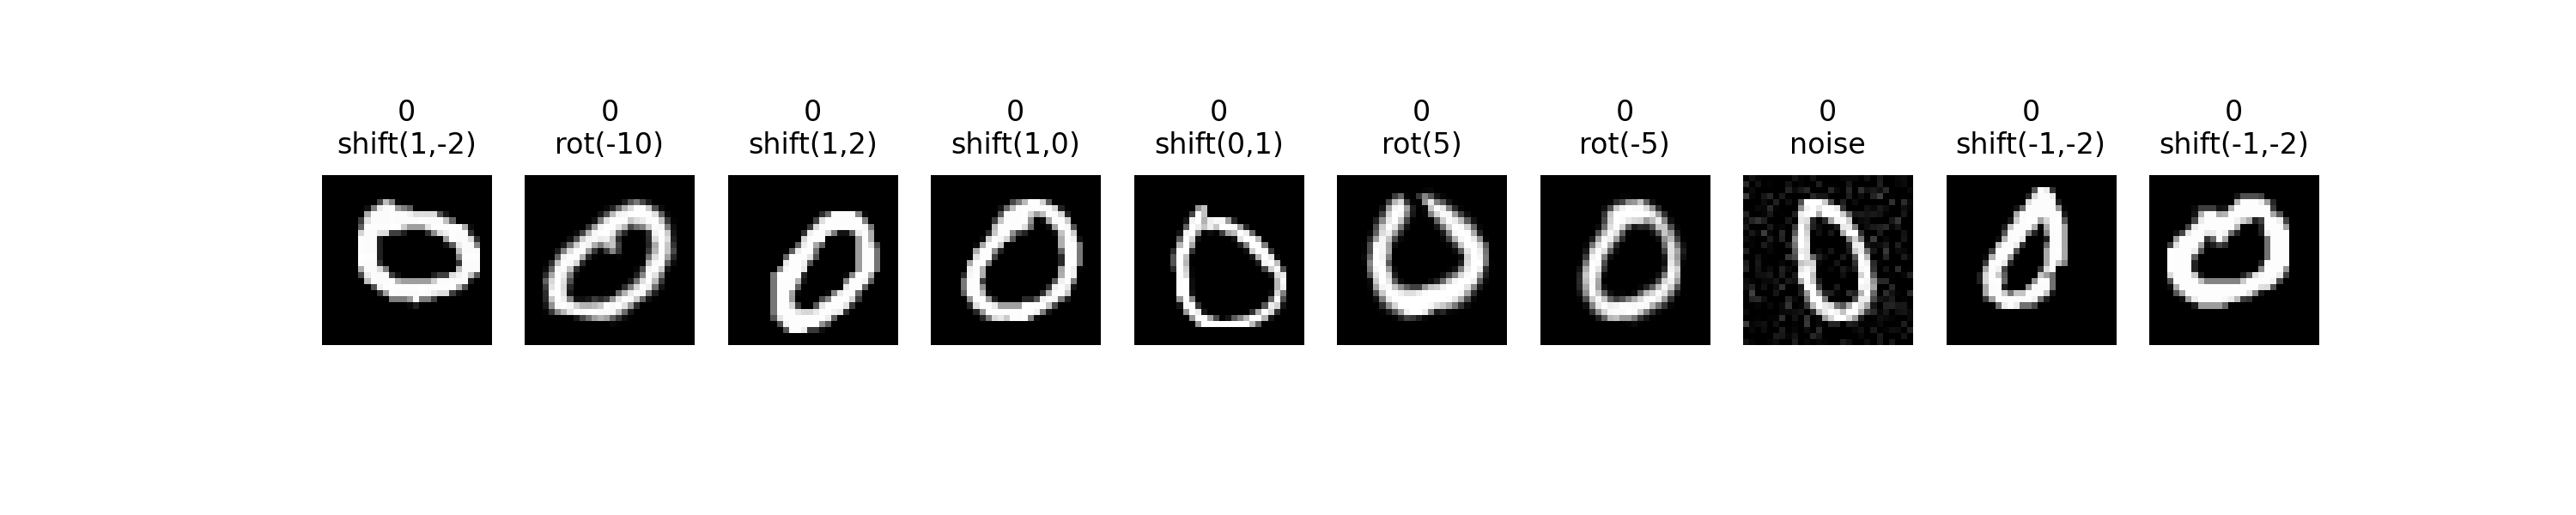
\includegraphics[width=0.8\textwidth]{Figures/P5/aug_350_1000.png}
\caption{Examples of augmented MNIST digits}
\label{fig:p5_augmentation}
\end{figure}

\subsection{Model Training}

A LeNet-5 convolutional neural network is used for classification. 
The model is trained using different combinations of real and augmented data.

Training is performed for 30 epochs with batch size 64. 
The training accuracy quickly reaches 100\%, indicating that the model can fully fit the training data.

\subsection{Training Progress}

Figure~\ref{fig:p5_training} shows the learning behavior of the model.
The loss decreases steadily while accuracy increases, demonstrating proper convergence.

\begin{figure}[htbp]
\centering
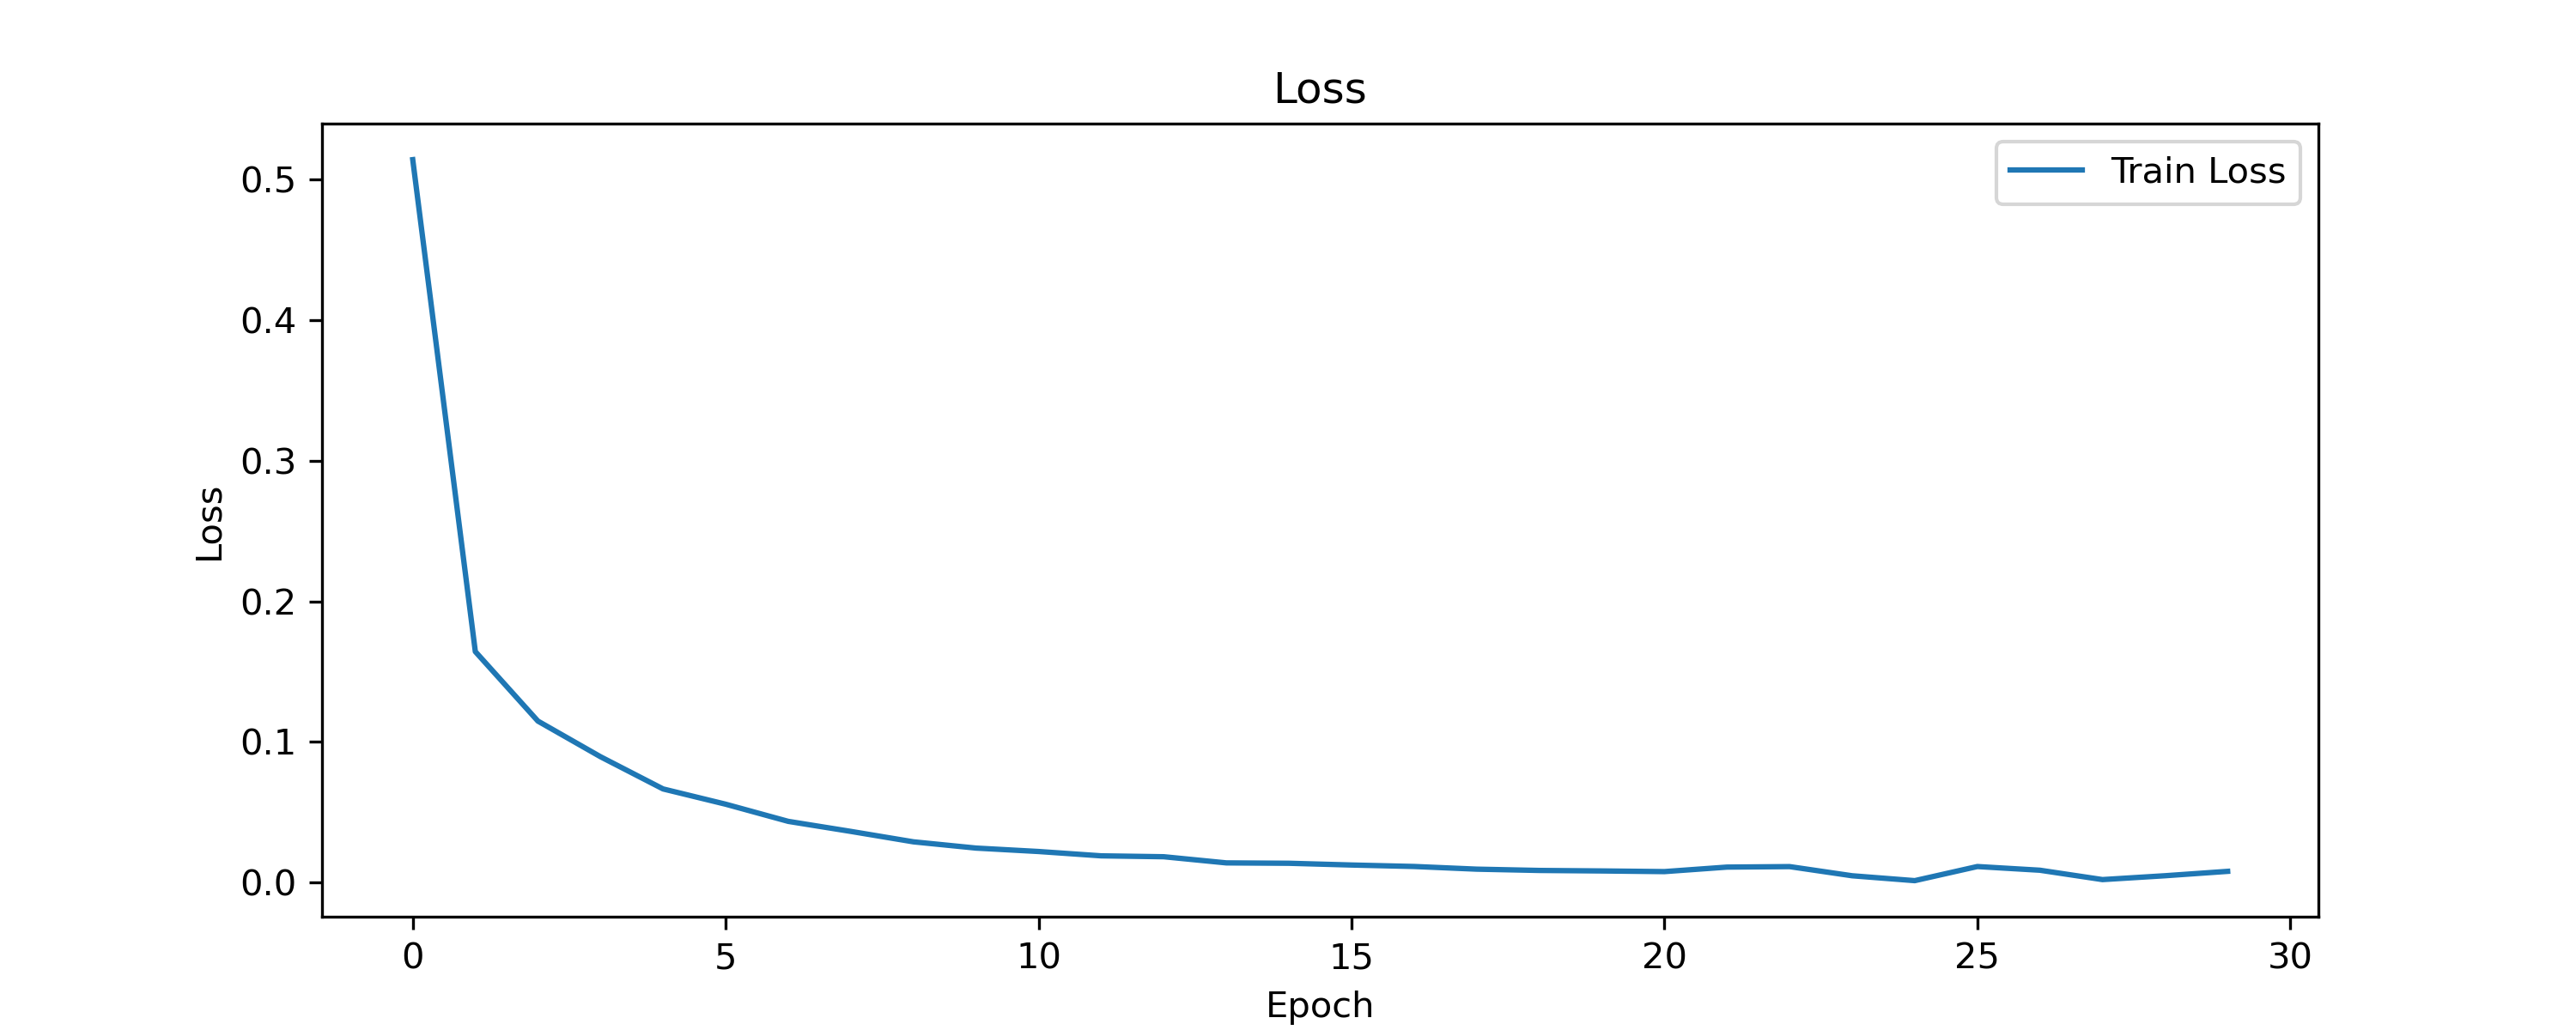
\includegraphics[width=0.7\textwidth]{Figures/P5/curve_1000_2000.png}
\caption{Training loss and accuracy curves}
\label{fig:p5_training}
\end{figure}

\subsection{Model Predictions}

Figure~\ref{fig:p5_predictions} shows sample predictions on the test dataset.
Correct predictions are shown in green, while incorrect ones are shown in red.

The model achieves high confidence in most predictions.

\begin{figure}[htbp]
\centering
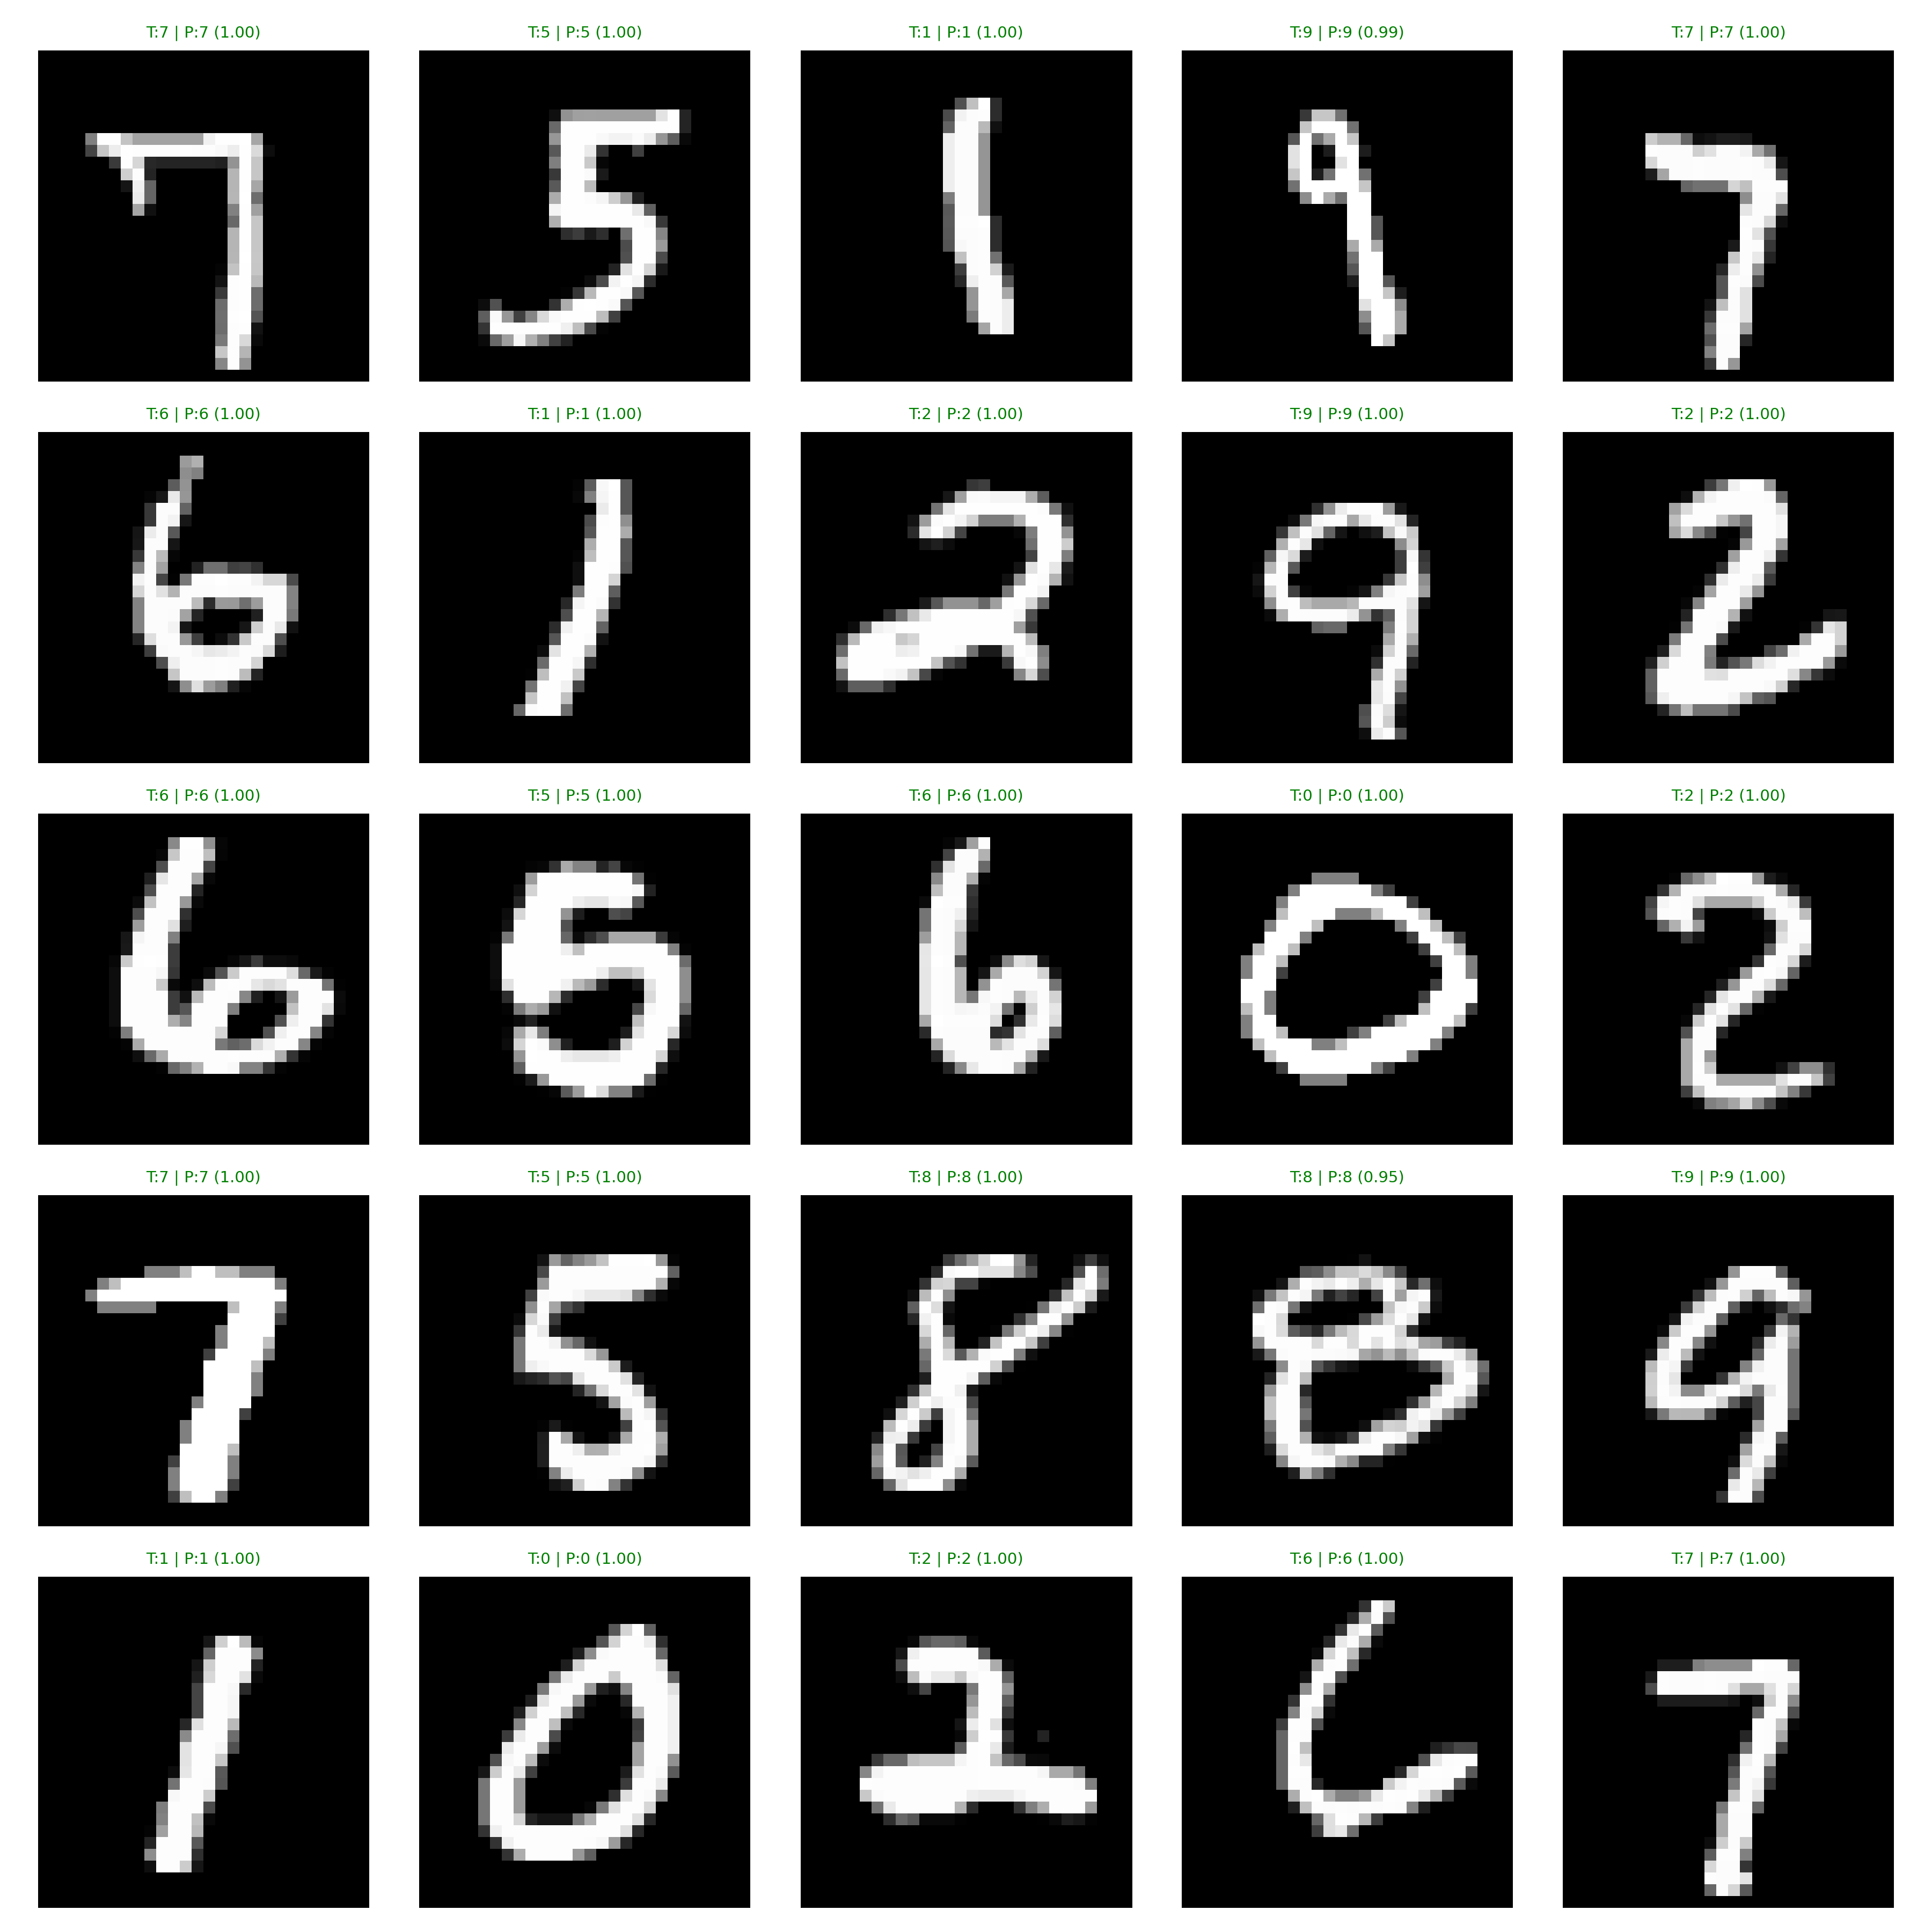
\includegraphics[width=0.7\textwidth]{Figures/P5/final_pred_1000_2000.png}
\caption{Model predictions on test samples}
\label{fig:p5_predictions}
\end{figure}

\subsection{Error Analysis}

Figure~\ref{fig:p5_errors} shows misclassified samples.
Most errors occur in visually ambiguous digits such as 3, 5, and 8.

This indicates that the model struggles with digits that have similar shapes.

\begin{figure}[htbp]
\centering
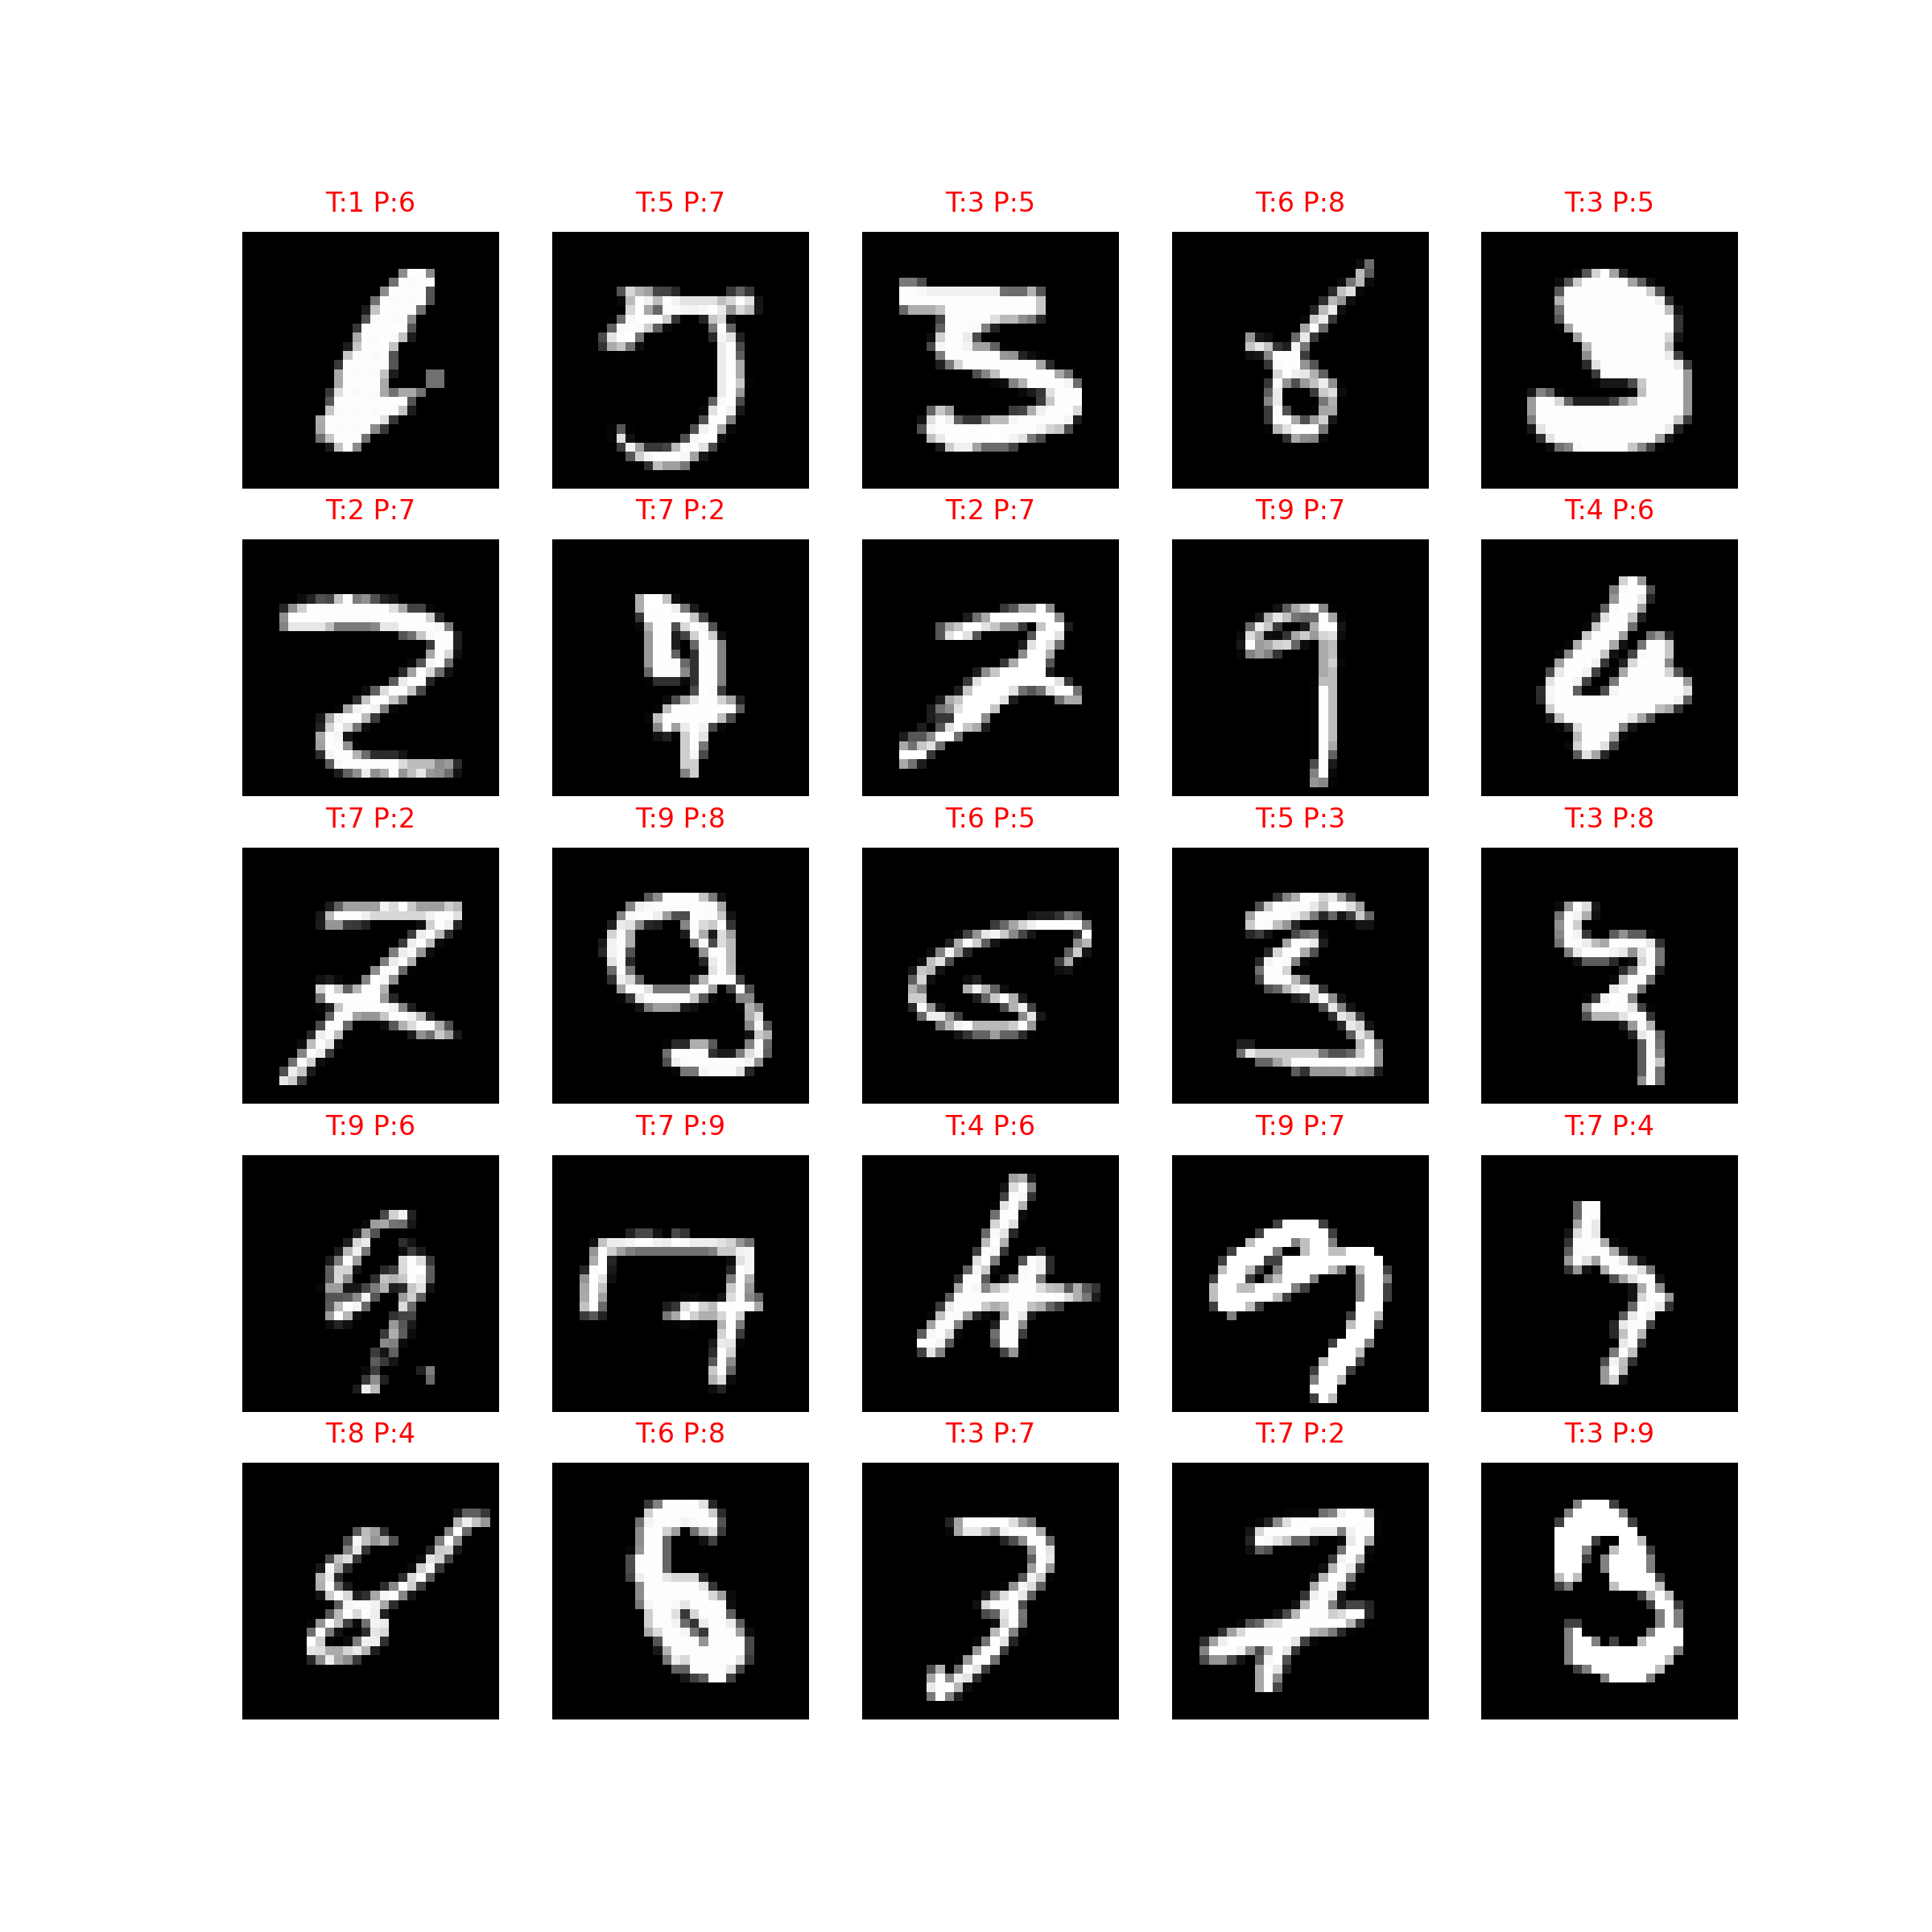
\includegraphics[width=0.7\textwidth]{Figures/P5/mis_1000_2000.png}
\caption{Misclassified test samples}
\label{fig:p5_errors}
\end{figure}

\section{Results and Discussion}

Figure~\ref{fig:p5_results} summarizes the performance of different configurations.

The best result achieved was:

\begin{itemize}
\item Accuracy = 98.01\%
\item Configuration: 350 real + 1000 augmented samples
\end{itemize}

This demonstrates that data augmentation significantly improves performance when the amount of real data is limited.

\begin{figure}[htbp]
\centering
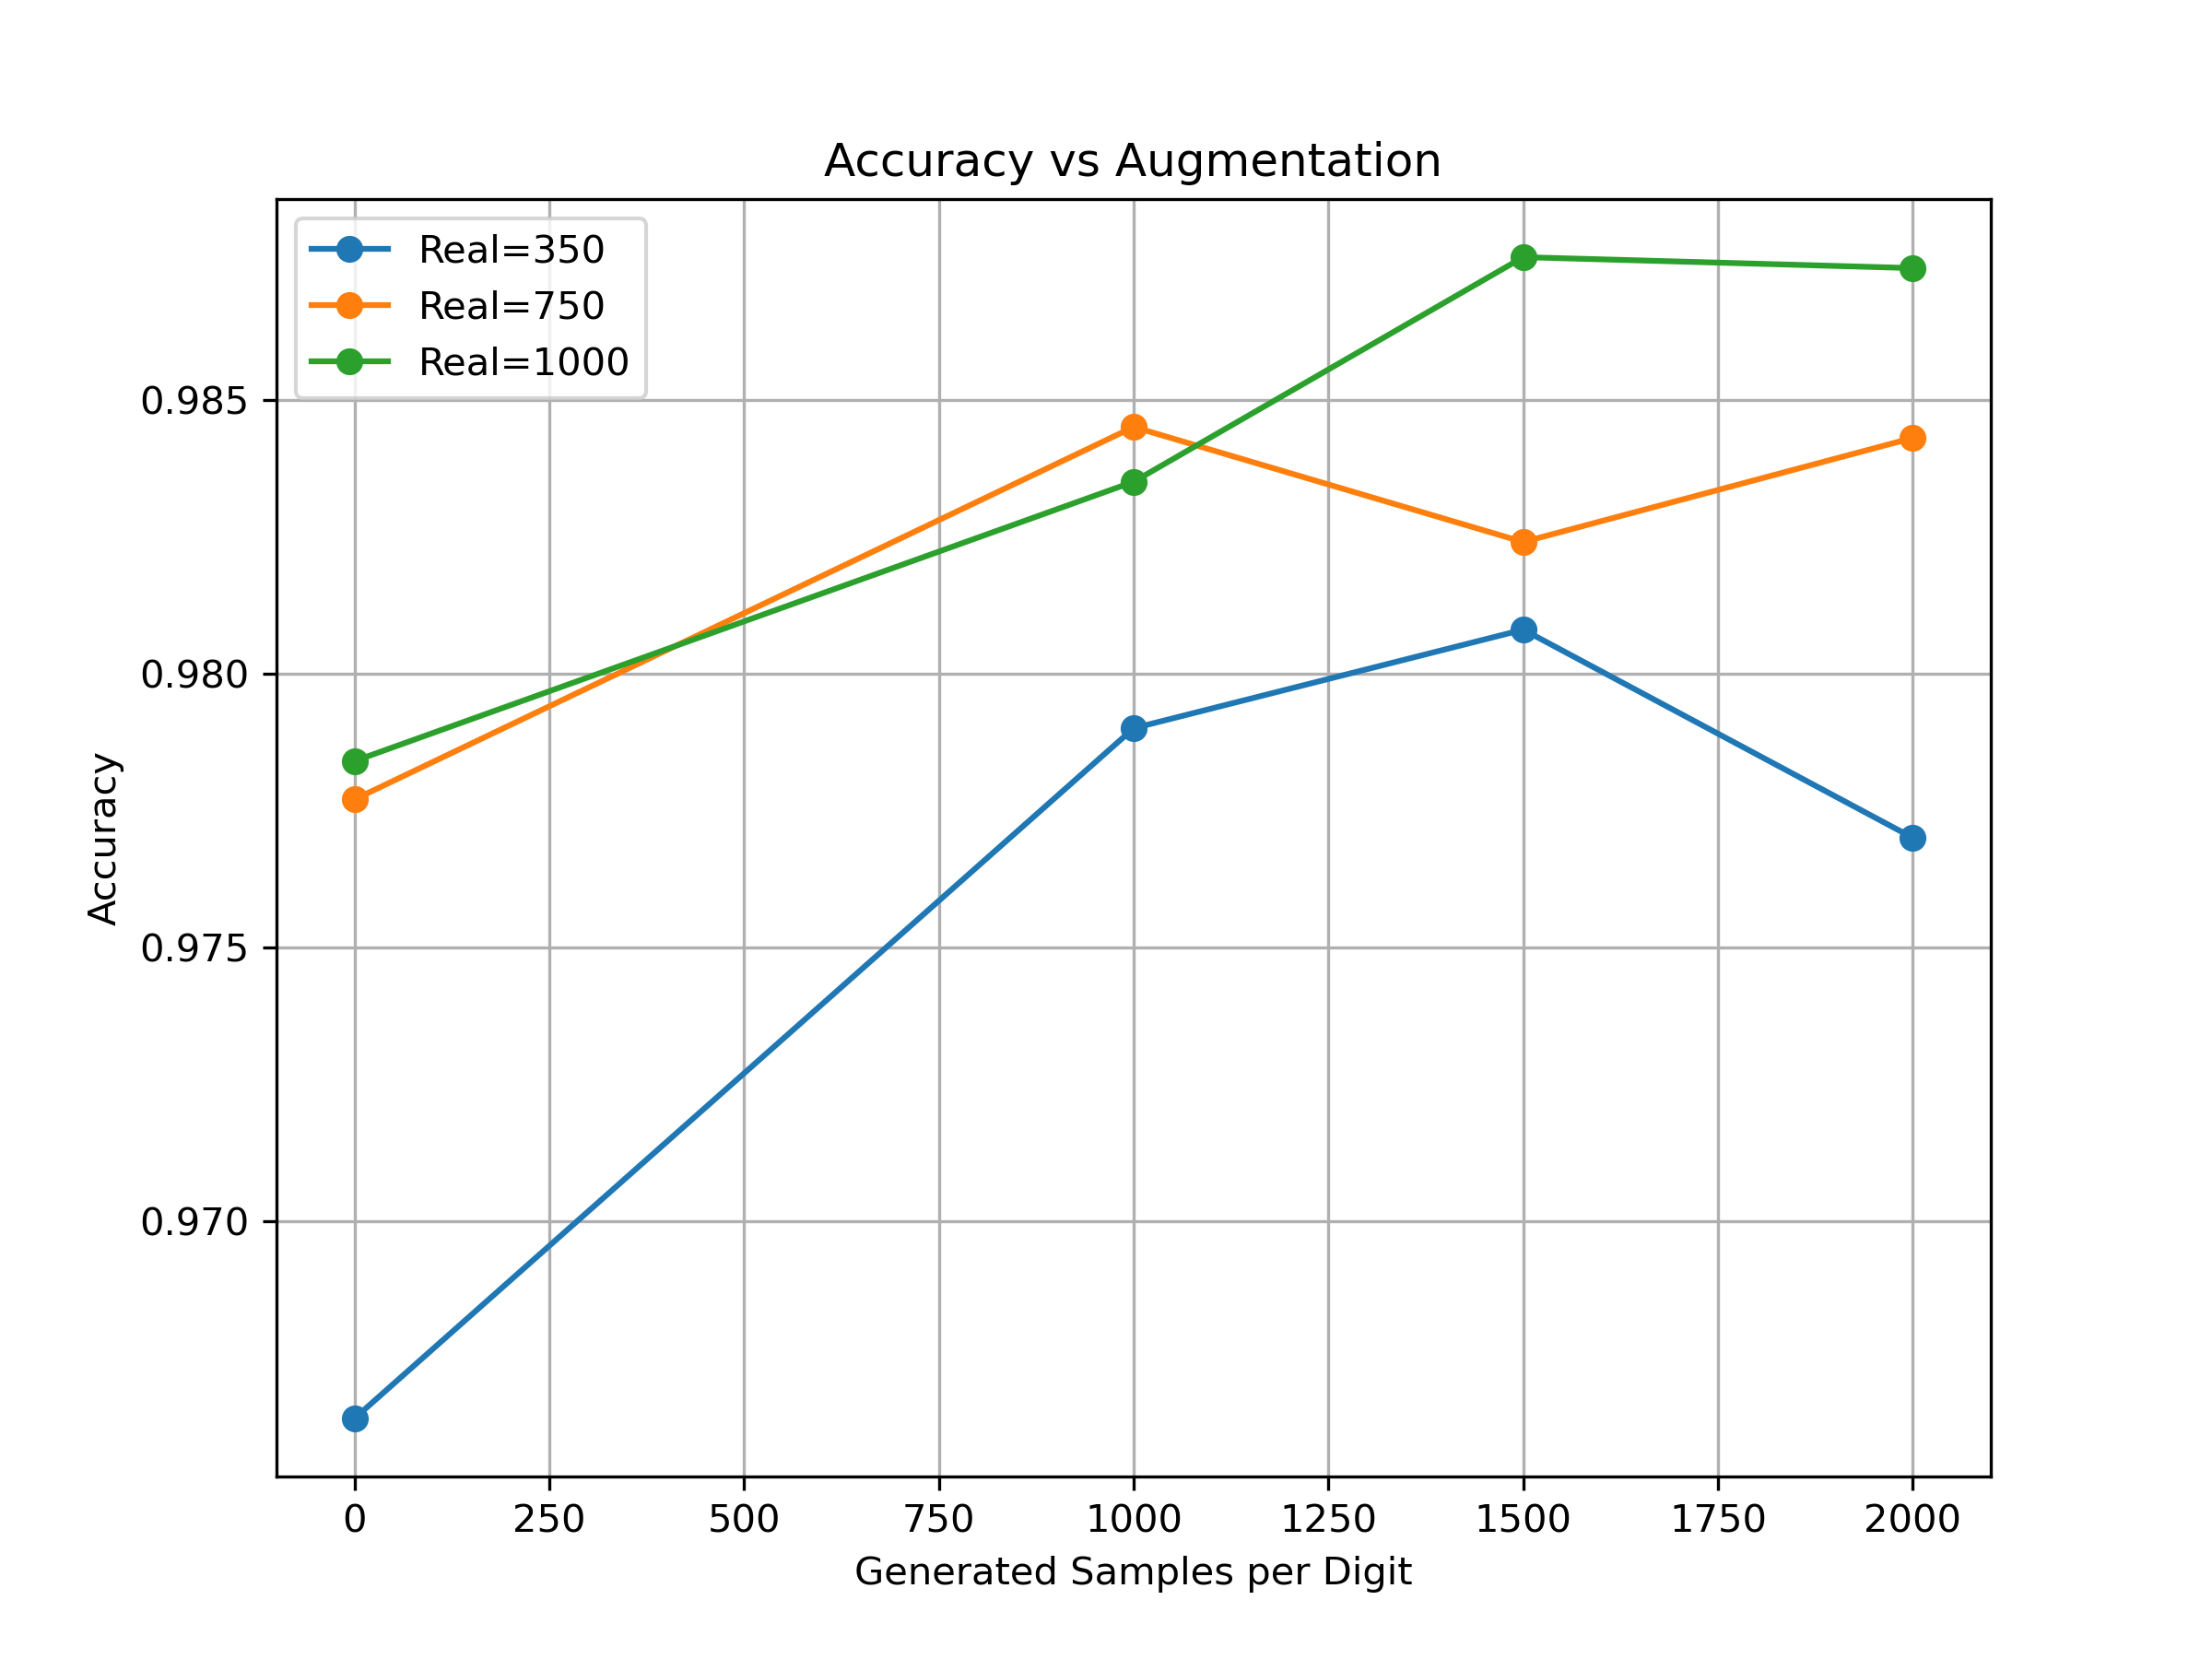
\includegraphics[width=0.7\textwidth]{Figures/P5/results_plot.png}
\caption{Accuracy vs number of augmented samples}
\label{fig:p5_results}
\end{figure}

\subsection{Key Observations}

\begin{itemize}
\item Increasing real data improves accuracy significantly.
\item Data augmentation helps most when real data is limited.
\item Excessive augmentation leads to diminishing returns.
\item The model achieves perfect training accuracy, indicating slight overfitting.
\item Test accuracy remains high, showing good generalization.
\end{itemize}


\end{document}